%
% absturz.tex -- Absturz eines Teilches in ein schwarzes Loch
%
\documentclass[tikz]{standalone}
\usepackage{times}
\usepackage{txfonts}
\usetikzlibrary{arrows,intersections}
\begin{document}
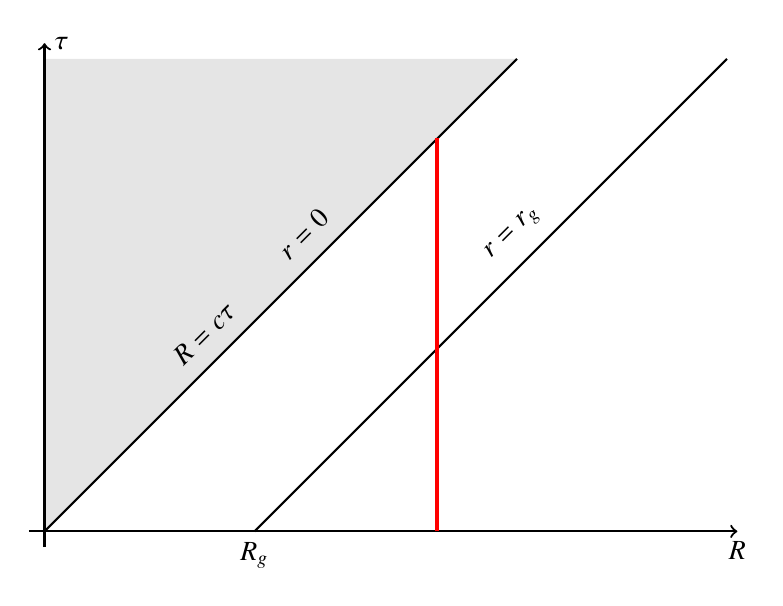
\begin{tikzpicture}[thick, scale = 4]
\coordinate (O) at (0,0);
\fill[gray!20] (0,0) -- (1.50,1.50) -- (0,1.50)--cycle;
\draw[->] (-0.05,0) -- (2.2,0) coordinate[label = {below:$R$}] (xmax);
\draw[->] (0,-0.05) -- (0,1.55) coordinate[label = {right:$\tau$}] (ymax);
\draw (0,0)--(1.50,1.50);
\draw (0.6666,0)--(2.16666,1.5);
\draw [line width = 1.5, red] (1.2474,0)--(1.2474,1.2474);
\node [label={[rotate=45] $R=c\tau$}] at (0.55,0.55) {};
\node [label={[rotate=45] $r=0$}] at (0.866,0.866) {};
\node [label={[rotate=45] $r=r_g$}] at (1.533,0.866) {};
\node [label={below:$R_g$}] at (0.6666,0.03) {};
\end{tikzpicture}
\end{document}

